\documentclass[tikz,border=4pt]{standalone}
\usepackage[T1]{fontenc}
\usepackage{lmodern}
\usetikzlibrary{arrows.meta,positioning,fit,backgrounds,calc}
\begin{document}
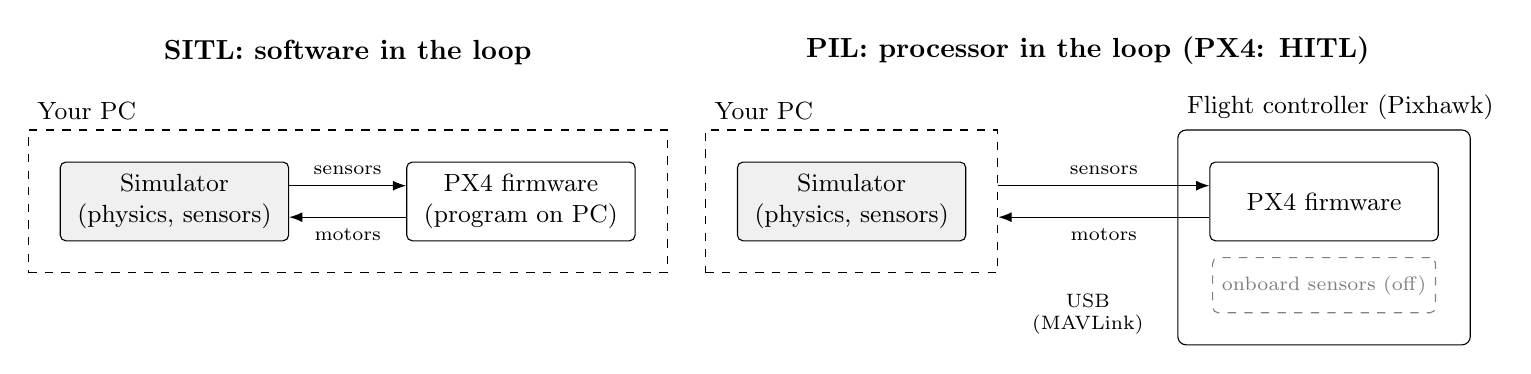
\begin{tikzpicture}[
  blk/.style={draw,rounded corners=2pt,minimum height=10mm,minimum width=29mm,align=center,font=\small,fill=white},
  ext/.style={blk,fill=gray!12},
  off/.style={blk,dashed,text=gray,draw=gray,minimum width=24mm,minimum height=7mm,font=\scriptsize},
  box/.style={draw,dashed,inner sep=4mm},
  lab/.style={font=\scriptsize,fill=white,inner sep=1pt,align=center},
  ttl/.style={font=\bfseries},
  >={Latex}]
% SITL
\node[ext] (sim1) at (0,0) {Simulator\\(physics, sensors)};
\node[blk] (px1) at (4.4,0) {PX4 firmware\\(program on PC)};
\begin{scope}[on background layer]
\node[box,fit=(sim1)(px1)] (pc1) {};
\end{scope}
\node[font=\small,anchor=south west] at (pc1.north west) {Your PC};
\draw[->] ($(sim1.east)+(0,2mm)$) -- node[lab,above=1mm]{sensors} ($(px1.west)+(0,2mm)$);
\draw[<-] ($(sim1.east)+(0,-2mm)$) -- node[lab,below=1mm]{motors} ($(px1.west)+(0,-2mm)$);
% PIL
\node[ext] (sim2) at (8.6,0) {Simulator\\(physics, sensors)};
\begin{scope}[on background layer]
\node[box,fit=(sim2)] (pc2) {};
\end{scope}
\node[font=\small,anchor=south west] at (pc2.north west) {Your PC};
\node[blk] (px2) at (14.6,0) {PX4 firmware};
\node[off,below=2mm of px2] (sen) {onboard sensors (off)};
\begin{scope}[on background layer]
\node[box,solid,rounded corners=3pt,fit=(px2)(sen)] (fc) {};
\end{scope}
\node[font=\small,anchor=south west] at (fc.north west) {Flight controller (Pixhawk)};
\draw[->] ($(pc2.east)+(0,2mm)$) -- node[lab,above=1mm]{sensors} ($(px2.west)+(0,2mm)$);
\draw[<-] ($(pc2.east)+(0,-2mm)$) -- node[lab,below=1mm]{motors} ($(px2.west)+(0,-2mm)$);
\node[lab] at ($(pc2.east)!0.5!(fc.west)+(0,-12mm)$) {USB\\(MAVLink)};
\node[ttl,anchor=south] at ($(pc1.north)+(0,7mm)$) {SITL: software in the loop};
\node[ttl,anchor=south] at ($(pc2.north west)!0.5!(fc.north east)+(0,7mm)$) {PIL: processor in the loop (PX4: HITL)};
\end{tikzpicture}
\end{document}
